\documentclass[12pt,a4paper]{ctexart}
\usepackage{graphicx}
\usepackage{wrapfig}
\usepackage{float}
\usepackage{siunitx}
\usepackage{subfigure}
\usepackage{caption}
\usepackage{natbib}
\usepackage{listings} % 引入listings宏包用于插入代码
\usepackage{xcolor} % 引入xcolor宏包以支持更多的颜色设置

% 设置Verilog代码样式
\lstdefinestyle{verilog}{
    language=Verilog, % 设置语言为Verilog
    basicstyle=\small\ttfamily, % 设置基本字体样式
    keywordstyle=\color{blue}, % 关键字颜色设置
    commentstyle=\color{gray}\ttfamily, % 注释颜色和样式设置
    stringstyle=\color{red!60!black},
    numbers=left, % 行号在左边显示
    numberstyle=\tiny,
    frame=single, % 添加单线框
    rulecolor=\color{black!30}, % 边框颜色
    breaklines=true, % 允许自动换行
}

\title{实验 6:完整流水线 CPU}
\author{张子康 \ PB22020660}
\date{\today}

\begin{document}
\maketitle
\newpage
\section{实验目的与内容}
\subsection{实验目的}
将结合前递模块与段间寄存器控制模块,得到一个能正常运行的完整流水线 CPU。
\subsection{实验内容}
\subsubsection{任务 1:前递模块}
根据实验文档的内容,根据传入的信号与优先级的判断,正确进行前递模块的设计。
\subsubsection{任务 2:加入前递的流水线}
将前递模块正确接入 CPU,形成加入前递的流水线,并通过对应仿真测试。
\subsubsection{任务 3:段间寄存器控制模块}
根据实验文档的内容,根据传入的信号,正确根据输入信号进行段间寄存器的控制模块设计。
\subsubsection{任务 4:完整流水线 CPU}
将段间寄存器控制模块正确接入 CPU,形成最终的流水线 CPU,并通过仿真、上板测试。
\section{逻辑设计}
\subsection{任务 1:前递模块}
\begin{lstlisting}[style=verilog]
module FORWARDING (
    input [0:0] rf_we_mem,
    input [0:0] rf_we_wb,
    input [4:0] rf_wa_mem,
    input [4:0] rf_wa_wb,
    input [31:0] rf_wd_mem,
    input [31:0] rf_wd_wb,
    input [4:0] rf_ra0_ex,
    input [4:0] rf_ra1_ex,
    output [0:0] rf_rd0_fe,
    output [0:0] rf_rd1_fe,
    output [31:0] rf_rd0_fd,
    output [31:0] rf_rd1_fd
);
    reg [31:0] rd0_fd,rd1_fd;
    reg [0:0] rd0_fe,rd1_fe;
    initial begin
        rd0_fd=0;
        rd0_fe=0;
        rd1_fd=0;
        rd1_fe=0;
    end

    assign rf_rd0_fe=rd0_fe;
    assign rf_rd1_fe=rd1_fe;
    assign rf_rd0_fd=rd0_fd;
    assign rf_rd1_fd=rd1_fd;

    always @(*) begin
        // 默认不前递
        rd0_fd=0;
        rd1_fd=0;
        rd0_fe=0;
        rd1_fe=0;
        // 如果发现写入的地址与读取的地址相同就前递
        if(rf_we_wb && rf_wa_wb!=5'b00000 && rf_wa_wb==rf_ra0_ex) begin
            rd0_fd=rf_wd_wb;
            rd0_fe=1;
        end 
        if(rf_we_wb && rf_wa_wb!=5'b00000 && rf_wa_wb==rf_ra1_ex) begin
            rd1_fd=rf_wd_wb;
            rd1_fe=1;
        end 
        if(rf_we_mem && rf_wa_mem!=5'b00000 && rf_wa_mem==rf_ra0_ex) begin
            rd0_fd=rf_wd_mem;
            rd0_fe=1;
        end 
        if(rf_we_mem && rf_wa_mem!=5'b00000 && rf_wa_mem==rf_ra1_ex) begin
            rd1_fd=rf_wd_mem;
            rd1_fe=1;
        end 
    end
endmodule
\end{lstlisting}
\subsection{任务 2:加入前递的流水线}
\begin{lstlisting}[style=verilog]
    // rf_rd0_ex_和rf_rd1_ex_为前递选择后的数据
    FORWARDING forwarding(
        .rf_we_mem(rf_we_mem),
        .rf_we_wb(rf_we_wb),
        .rf_wa_mem(rf_wa_mem),
        .rf_wa_wb(rf_wa_wb),
        .rf_wd_mem(alu_res_mem),
        .rf_wd_wb(alu_res_wb),
        .rf_ra0_ex(rf_ra0_ex),
        .rf_ra1_ex(rf_ra1_ex),
        .rf_rd0_fe(rf_rd0_fe),
        .rf_rd1_fe(rf_rd1_fe),
        .rf_rd0_fd(rf_rd0_fd),
        .rf_rd1_fd(rf_rd1_fd)
    );

    MUX1 mux3(
        .src1(rf_rd0_fd),
        .src0(rf_rd0_ex),
        .sel(rf_rd0_fe),
        .res(rf_rd0_ex_)
    );

    MUX1 mux4(
        .src1(rf_rd1_fd),
        .src0(rf_rd1_ex),
        .sel(rf_rd1_fe),
        .res(rf_rd1_ex_)
    );
\end{lstlisting}
将上述代码加入CPU模块,同时作出如下修改:
\begin{lstlisting}[style=verilog]
    MUX1 mux1(
        .src0(rf_rd0_ex_),
        .src1(pc_ex),
        .sel(alu_src0_sel_ex),
        .res(alu_src0_ex)
    );

    MUX1 mux2(
        .src0(rf_rd1_ex_),
        .src1(imm_ex),
        .sel(alu_src1_sel_ex),
        .res(alu_src1_ex)
    );

    EX_MEM ex_mem(
        .clk(clk),
        .rst(rst),
        .flush(flush_ex_mem),
        .stall(stall),
        .en(en),
        //PC
        .pc_add4_in(pcadd4_ex),
        .pc_in(pc_ex),
        .pc_add4_out(pcadd4_mem),
        .pc_out(pc_mem),
        //INST
        .inst_in(inst_ex),
        .inst_out(inst_mem),
        //DECODER
        .alu_op_in(alu_op_ex),
        .dmem_access_in(dmem_access_ex),
        .imm_in(imm_ex),
        .rf_ra0_in(rf_ra0_ex),
        .rf_ra1_in(rf_ra1_ex),
        .rf_wa_in(rf_wa_ex),
        .rf_we_in(rf_we_ex),
        .rf_wd_sel_in(rf_wd_sel_ex),
        .alu_src0_sel_in(alu_src0_sel_ex),
        .alu_src1_sel_in(alu_src1_sel_ex),
        .br_type_in(br_type_ex),
        .dmem_we_in(dmem_we_ex),
        .alu_op_out(alu_op_mem),
        .dmem_access_out(dmem_access_mem),
        .imm_out(imm_mem),
        .rf_ra0_out(rf_ra0_mem),
        .rf_ra1_out(rf_ra1_mem),
        .rf_wa_out(rf_wa_mem),
        .rf_we_out(rf_we_mem),
        .rf_wd_sel_out(rf_wd_sel_mem),
        .alu_src0_sel_out(alu_src0_sel_mem),
        .alu_src1_sel_out(alu_src1_sel_mem),
        .br_type_out(br_type_mem),
        .dmem_we_out(dmem_we_mem),
        //REG_FILE
        .rf_rd0_in(rf_rd0_ex_),
        .rf_rd1_in(rf_rd1_ex_),
        .rf_rd0_out(rf_rd0_mem),
        .rf_rd1_out(rf_rd1_mem),
        //MUX1
        .alu_src0_in(alu_src0_ex),
        .alu_src1_in(alu_src1_ex),
        .alu_src0_out(alu_src0_mem),
        .alu_src1_out(alu_src1_mem),
        //NPC
        .npc_in(npc_ex),
        .npc_out(npc_mem),
        //BRANCH
        .npc_sel_in(npc_sel_ex),
        .npc_sel_out(npc_sel_mem),
        //ALU
        .alu_res_in(alu_res_ex),
        .alu_res_out(alu_res_mem),
        //SLU
        .dmem_rd_out_in(0),
        .dmem_wdata_mem_in(0),
        .dmem_rd_out_out(),
        .dmem_wdata_mem_out(),
        //DM
        .dmem_rdata_mem_in(0),
        .dmem_rdata_mem_out(),
        .commit_in(commit_ex),
        .commit_out(commit_mem)
    );
\end{lstlisting}
\subsection{任务 3:段间寄存器控制模块}
\begin{lstlisting}[style=verilog]
`define DMEM_RDATA 2'b10
module SEG_CTRL (
    input [0:0] rf_we_ex,
    input [1:0] rf_wd_sel_ex,
    input [4:0] rf_wa_ex,
    input [4:0] rf_ra0_id,
    input [4:0] rf_ra1_id,
    input [1:0] npc_sel_ex,
    output reg [0:0] stall_pc,
    output reg [0:0] stall_if_id,
    output reg [0:0] flush_if_id,
    output reg [0:0] flush_id_ex
);
    always @(*) begin
        // 默认不阻塞或冲刷流水线
        stall_pc=0;
        stall_if_id=0;
        flush_id_ex=0;
        flush_if_id=0;
        // 对于load-use,若写入地址和读取地址相同
        // 则阻塞流水线2周期
        if(rf_we_ex && rf_wd_sel_ex==`DMEM_RDATA && (rf_wa_ex==rf_ra0_id || rf_wa_ex==rf_ra1_id))begin
            flush_id_ex=1'b1;
            stall_pc=1'b1;
            stall_if_id=1'b1;
        end
        // 对于跳转指令,直接冲刷流水线
        if(npc_sel_ex!=2'b00) begin
            flush_id_ex=1'b1;
            flush_if_id=1'b1;
        end
    end
endmodule
\end{lstlisting}
\subsection{任务 4:完整流水线 CPU}
\begin{lstlisting}[style=verilog]
`include "./include/config.v"

module CPU (input [0 : 0] clk,
            input [0 : 0] rst,
            input [0 : 0] global_en,
            output [31 : 0] imem_raddr,
            input [31 : 0] imem_rdata,
            input [31 : 0] dmem_rdata,      // Unused
            output [0 : 0] dmem_we,        // Unused
            output [31 : 0] dmem_addr,      // Unused
            output [31 : 0] dmem_wdata,     // Unused
            output [0 : 0] commit,
            output [31 : 0] commit_pc,
            output [31 : 0] commit_inst,
            output [0 : 0] commit_halt,
            output [0 : 0] commit_reg_we,
            output [4 : 0] commit_reg_wa,
            output [31 : 0] commit_reg_wd,
            output [0 : 0] commit_dmem_we,
            output [31 : 0] commit_dmem_wa,
            output [31 : 0] commit_dmem_wd,
            input [4 : 0] debug_reg_ra,
            output [31 : 0] debug_reg_rd);
    
    
    // TODO
    wire [0:0] commit_if;
    wire [31:0] pc_if;
    wire [31:0] pcadd4_if;
    wire [31:0] inst_if;
    
    wire [0:0] commit_id;
    wire [31:0] pc_id;
    wire [31:0] pcadd4_id;
    wire [31:0] inst_id;
    wire [4:0] alu_op_id;
    wire [3:0] dmem_access_id;
    wire [31:0] imm_id;
    wire [4:0] rf_ra0_id;
    wire [4:0] rf_ra1_id;
    wire [5:0] rf_wa_id;
    wire [0:0] rf_we_id;
    wire [1:0] rf_wd_sel_id;
    wire [0:0] alu_src0_sel_id;
    wire [0:0] alu_src1_sel_id;
    wire [3:0] br_type_id;
    wire [0:0] dmem_we_id;
    wire [31:0] rf_rd0_id;
    wire [31:0] rf_rd1_id;

    wire [0:0] commit_ex;
    wire [31:0] pc_ex;
    wire [31:0] pcadd4_ex;
    wire [31:0] inst_ex;
    wire [4:0] alu_op_ex;
    wire [3:0] dmem_access_ex;
    wire [31:0] imm_ex;
    wire [4:0] rf_ra0_ex;
    wire [4:0] rf_ra1_ex;
    wire [5:0] rf_wa_ex;
    wire [0:0] rf_we_ex;
    wire [1:0] rf_wd_sel_ex;
    wire [0:0] alu_src0_sel_ex;
    wire [0:0] alu_src1_sel_ex;
    wire [3:0] br_type_ex;
    wire [0:0] dmem_we_ex;
    wire [31:0] rf_rd0_ex;
    wire [31:0] rf_rd1_ex;
    wire [31:0] npc_ex;
    wire [31:0] pc_j_ex;
    wire [31:0] alu_src0_ex;
    wire [31:0] alu_src1_ex;
    wire [31:0] alu_res_ex;
    wire [1:0] npc_sel_ex;

    wire [0:0] commit_mem;
    wire [31:0] pc_mem;
    wire [31:0] pcadd4_mem;
    wire [31:0] inst_mem;
    wire [4:0] alu_op_mem;
    wire [3:0] dmem_access_mem;
    wire [31:0] imm_mem;
    wire [4:0] rf_ra0_mem;
    wire [4:0] rf_ra1_mem;
    wire [5:0] rf_wa_mem;
    wire [0:0] rf_we_mem;
    wire [1:0] rf_wd_sel_mem;
    wire [0:0] alu_src0_sel_mem;
    wire [0:0] alu_src1_sel_mem;
    wire [3:0] br_type_mem;
    wire [0:0] dmem_we_mem;
    wire [31:0] rf_rd0_mem;
    wire [31:0] rf_rd1_mem;
    wire [31:0] npc_mem;
    wire [31:0] pc_j_mem;
    wire [31:0] alu_src0_mem;
    wire [31:0] alu_src1_mem;
    wire [31:0] alu_res_mem;
    wire [31:0] dmem_rd_out_mem;
    wire [31:0] dmem_wdata_mem;
    wire [31:0] dmem_rdata_mem;
    wire [1:0] npc_sel_mem;

    wire [0:0] commit_wb;
    wire [31:0] pc_wb;
    wire [31:0] pcadd4_wb;
    wire [31:0] inst_wb;
    wire [4:0] alu_op_wb;
    wire [3:0] dmem_access_wb;
    wire [31:0] imm_wb;
    wire [4:0] rf_ra0_wb;
    wire [4:0] rf_ra1_wb;
    wire [5:0] rf_wa_wb;
    wire [0:0] rf_we_wb;
    wire [1:0] rf_wd_sel_wb;
    wire [0:0] alu_src0_sel_wb;
    wire [0:0] alu_src1_sel_wb;
    wire [3:0] br_type_wb;
    wire [0:0] dmem_we_wb;
    wire [31:0] rf_rd0_wb;
    wire [31:0] rf_rd1_wb;
    wire [31:0] npc_wb;
    wire [31:0] pc_j_wb;
    wire [31:0] alu_src0_wb;
    wire [31:0] alu_src1_wb;
    wire [31:0] alu_res_wb;
    wire [31:0] dmem_rd_out_wb;
    wire [31:0] dmem_wdata_wb;
    wire [31:0] dmem_rdata_wb;
    wire [31:0] rf_wd_wb;
    wire [1:0] npc_sel_wb;

    wire [0:0] rf_rd0_fe,rf_rd1_fe;
    wire [31:0] rf_rd0_fd,rf_rd1_fd;
    wire [31:0] rf_rd0_ex_,rf_rd1_ex_;

    wire flush,stall,stall_pc,stall_if_id,en;
    wire flush_if_id,flush_id_ex,flush_ex_mem,flush_mem_wb;

    assign commit_if = 1;
    assign stall = 0;
    assign en = global_en;
    assign global_en  = !(inst_wb == 32'H00100073);
    assign imem_raddr = (pc_if-32'h00400000)/'d4;
    assign inst_if   = imem_rdata;
    assign pc_j_ex       = alu_res_ex&~1;
    assign dmem_wd_in = rf_rd1_mem;
    assign dmem_we    = dmem_we_mem;
    assign dmem_addr  = (alu_res_mem-32'h10010000)/'d4;
    assign dmem_wdata = dmem_wdata_mem;
    assign dmem_rdata_mem = dmem_rdata;
    //assign flush_if_id=inst_if==32'h00000013 && inst_id==32'h00000013;
    //assign flush_id_ex=inst_if==32'h00000013 && inst_id==32'h00000013;
    assign flush_ex_mem=0;
    assign flush_mem_wb=0;

    // 前递模块
    FORWARDING forwarding(
        .rf_we_mem(rf_we_mem),
        .rf_we_wb(rf_we_wb),
        .rf_wa_mem(rf_wa_mem),
        .rf_wa_wb(rf_wa_wb),
        .rf_wd_mem(alu_res_mem),
        .rf_wd_wb(alu_res_wb),
        .rf_ra0_ex(rf_ra0_ex),
        .rf_ra1_ex(rf_ra1_ex),
        .rf_rd0_fe(rf_rd0_fe),
        .rf_rd1_fe(rf_rd1_fe),
        .rf_rd0_fd(rf_rd0_fd),
        .rf_rd1_fd(rf_rd1_fd)
    );

    MUX1 mux3(
        .src1(rf_rd0_fd),
        .src0(rf_rd0_ex),
        .sel(rf_rd0_fe),
        .res(rf_rd0_ex_)
    );

    MUX1 mux4(
        .src1(rf_rd1_fd),
        .src0(rf_rd1_ex),
        .sel(rf_rd1_fe),
        .res(rf_rd1_ex_)
    );

    // 段间寄存器控制器
    SEG_CTRL seg_ctrl(
        .rf_we_ex(rf_we_ex),
        .rf_wd_sel_ex(rf_wd_sel_ex),
        .rf_wa_ex(rf_wa_ex),
        .rf_ra0_id(rf_ra0_id),
        .rf_ra1_id(rf_ra1_id),
        .npc_sel_ex(npc_sel_ex),
        .stall_pc(stall_pc),
        .stall_if_id(stall_if_id),
        .flush_if_id(flush_if_id),
        .flush_id_ex(flush_id_ex)
    );


    PC_PLUS4 pc_plus(
        .pc(pc_if),
        .pc_plus4(pcadd4_if)
    );
    
    PC pc(
        .clk    (clk),
        .rst    (rst),
        .en     (global_en),    // 当 global_en 为高电平时,PC 才会更新,CPU 才会执行指令。
        .npc    (npc_ex),
        .pc     (pc_if),
        .stall (stall_pc),
        .flush(flush)
    );

    IF_ID if_id(
        .clk(clk),
        .rst(rst),
        .flush(flush_if_id),
        .stall(stall_if_id),
        .en(en),
        //PC
        .pc_add4_in(pcadd4_if),
        .pc_in(pc_if),
        .pc_add4_out(pcadd4_id),
        .pc_out(pc_id),
        //INST
        .inst_in(inst_if),
        .inst_out(inst_id),
        //DECODER
        .alu_op_in(0),
        .dmem_access_in(0),
        .imm_in(0),
        .rf_ra0_in(0),
        .rf_ra1_in(0),
        .rf_wa_in(0),
        .rf_we_in(0),
        .rf_wd_sel_in(0),
        .alu_src0_sel_in(0),
        .alu_src1_sel_in(0),
        .br_type_in(0),
        .dmem_we_in(0),
        .alu_op_out(),
        .dmem_access_out(),
        .imm_out(),
        .rf_ra0_out(),
        .rf_ra1_out(),
        .rf_wa_out(),
        .rf_we_out(),
        .rf_wd_sel_out(),
        .alu_src0_sel_out(),
        .alu_src1_sel_out(),
        .br_type_out(),
        .dmem_we_out(),
        //REG_FILE
        .rf_rd0_in(0),
        .rf_rd1_in(0),
        .rf_rd0_out(),
        .rf_rd1_out(),
        //MUX1
        .alu_src0_in(0),
        .alu_src1_in(0),
        .alu_src0_out(),
        .alu_src1_out(),
        //NPC
        .npc_in(0),
        .npc_out(),
        //BRANCH
        .npc_sel_in(0),
        .npc_sel_out(),
        //ALU
        .alu_res_in(0),
        .alu_res_out(),
        //SLU
        .dmem_rd_out_in(0),
        .dmem_wdata_mem_in(0),
        .dmem_rd_out_out(),
        .dmem_wdata_mem_out(),
        //DM
        .dmem_rdata_mem_in(0),
        .dmem_rdata_mem_out(),
        .commit_in(commit_if),
        .commit_out(commit_id)
    );

    DECODER decoder(
        .inst(inst_id),
        .alu_op(alu_op_id),
        .imm(imm_id),
        .rf_ra0(rf_ra0_id),
        .rf_ra1(rf_ra1_id),
        .rf_wa(rf_wa_id),
        .rf_we(rf_we_id),
        .alu_src0_sel(alu_src0_sel_id),
        .alu_src1_sel(alu_src1_sel_id),
        .dmem_access(dmem_access_id),
        .rf_wd_sel(rf_wd_sel_id),
        .br_type(br_type_id),
        .dmem_we(dmem_we_id)
    );
    
    REG_FILE reg_file(
        .clk(clk),
        .rf_ra0(rf_ra0_id),
        .rf_ra1(rf_ra1_id),
        .rf_wa(rf_wa_wb),
        .rf_we(rf_we_wb),
        .rf_wd(rf_wd_wb),
        .rf_rd0(rf_rd0_id),
        .rf_rd1(rf_rd1_id),
        .debug_reg_rd(debug_reg_rd),
        .debug_reg_ra(debug_reg_ra)
    );
    
    ID_EX id_ex(
        .clk(clk),
        .rst(rst),
        .flush(flush_id_ex),
        .stall(stall),
        .en(en),
        //PC
        .pc_add4_in(pcadd4_id),
        .pc_in(pc_id),
        .pc_add4_out(pcadd4_ex),
        .pc_out(pc_ex),
        //INST
        .inst_in(inst_id),
        .inst_out(inst_ex),
        //DECODER
        .alu_op_in(alu_op_id),
        .dmem_access_in(dmem_access_id),
        .imm_in(imm_id),
        .rf_ra0_in(rf_ra0_id),
        .rf_ra1_in(rf_ra1_id),
        .rf_wa_in(rf_wa_id),
        .rf_we_in(rf_we_id),
        .rf_wd_sel_in(rf_wd_sel_id),
        .alu_src0_sel_in(alu_src0_sel_id),
        .alu_src1_sel_in(alu_src1_sel_id),
        .br_type_in(br_type_id),
        .dmem_we_in(dmem_we_id),
        .alu_op_out(alu_op_ex),
        .dmem_access_out(dmem_access_ex),
        .imm_out(imm_ex),
        .rf_ra0_out(rf_ra0_ex),
        .rf_ra1_out(rf_ra1_ex),
        .rf_wa_out(rf_wa_ex),
        .rf_we_out(rf_we_ex),
        .rf_wd_sel_out(rf_wd_sel_ex),
        .alu_src0_sel_out(alu_src0_sel_ex),
        .alu_src1_sel_out(alu_src1_sel_ex),
        .br_type_out(br_type_ex),
        .dmem_we_out(dmem_we_ex),
        //REG_FILE
        .rf_rd0_in(rf_rd0_id),
        .rf_rd1_in(rf_rd1_id),
        .rf_rd0_out(rf_rd0_ex),
        .rf_rd1_out(rf_rd1_ex),
        //MUX1
        .alu_src0_in(0),
        .alu_src1_in(0),
        .alu_src0_out(),
        .alu_src1_out(),
        //NPC
        .npc_in(0),
        .npc_out(),
        //BRANCH
        .npc_sel_in(0),
        .npc_sel_out(),
        //ALU
        .alu_res_in(0),
        .alu_res_out(),
        //SLU
        .dmem_rd_out_in(0),
        .dmem_wdata_mem_in(0),
        .dmem_rd_out_out(),
        .dmem_wdata_mem_out(),
        //DM
        .dmem_rdata_mem_in(0),
        .dmem_rdata_mem_out(),
        .commit_in(commit_id),
        .commit_out(commit_ex)
    );

    MUX1 mux1(
        .src0(rf_rd0_ex_),
        .src1(pc_ex),
        .sel(alu_src0_sel_ex),
        .res(alu_src0_ex)
    );

    MUX1 mux2(
        .src0(rf_rd1_ex_),
        .src1(imm_ex),
        .sel(alu_src1_sel_ex),
        .res(alu_src1_ex)
    );
    
    ALU alu(
        .alu_src0(alu_src0_ex),
        .alu_src1(alu_src1_ex),
        .alu_op(alu_op_ex),
        .alu_res(alu_res_ex)
    );
    
    BRANCH branch(
        .br_type(br_type_ex),
        .br_src0(rf_rd0_ex_),
        .br_src1(rf_rd1_ex_),
        .npc_sel(npc_sel_ex)
    );
    NPC npc(
        .pc_offset(alu_res_ex),
        .pc_add4(pcadd4_if),
        .pc_j(pc_j_ex),
        .npc_sel(npc_sel_ex),
        .npc(npc_ex)
    );

    EX_MEM ex_mem(
        .clk(clk),
        .rst(rst),
        .flush(flush_ex_mem),
        .stall(stall),
        .en(en),
        //PC
        .pc_add4_in(pcadd4_ex),
        .pc_in(pc_ex),
        .pc_add4_out(pcadd4_mem),
        .pc_out(pc_mem),
        //INST
        .inst_in(inst_ex),
        .inst_out(inst_mem),
        //DECODER
        .alu_op_in(alu_op_ex),
        .dmem_access_in(dmem_access_ex),
        .imm_in(imm_ex),
        .rf_ra0_in(rf_ra0_ex),
        .rf_ra1_in(rf_ra1_ex),
        .rf_wa_in(rf_wa_ex),
        .rf_we_in(rf_we_ex),
        .rf_wd_sel_in(rf_wd_sel_ex),
        .alu_src0_sel_in(alu_src0_sel_ex),
        .alu_src1_sel_in(alu_src1_sel_ex),
        .br_type_in(br_type_ex),
        .dmem_we_in(dmem_we_ex),
        .alu_op_out(alu_op_mem),
        .dmem_access_out(dmem_access_mem),
        .imm_out(imm_mem),
        .rf_ra0_out(rf_ra0_mem),
        .rf_ra1_out(rf_ra1_mem),
        .rf_wa_out(rf_wa_mem),
        .rf_we_out(rf_we_mem),
        .rf_wd_sel_out(rf_wd_sel_mem),
        .alu_src0_sel_out(alu_src0_sel_mem),
        .alu_src1_sel_out(alu_src1_sel_mem),
        .br_type_out(br_type_mem),
        .dmem_we_out(dmem_we_mem),
        //REG_FILE
        .rf_rd0_in(rf_rd0_ex_),
        .rf_rd1_in(rf_rd1_ex_),
        .rf_rd0_out(rf_rd0_mem),
        .rf_rd1_out(rf_rd1_mem),
        //MUX1
        .alu_src0_in(alu_src0_ex),
        .alu_src1_in(alu_src1_ex),
        .alu_src0_out(alu_src0_mem),
        .alu_src1_out(alu_src1_mem),
        //NPC
        .npc_in(npc_ex),
        .npc_out(npc_mem),
        //BRANCH
        .npc_sel_in(npc_sel_ex),
        .npc_sel_out(npc_sel_mem),
        //ALU
        .alu_res_in(alu_res_ex),
        .alu_res_out(alu_res_mem),
        //SLU
        .dmem_rd_out_in(0),
        .dmem_wdata_mem_in(0),
        .dmem_rd_out_out(),
        .dmem_wdata_mem_out(),
        //DM
        .dmem_rdata_mem_in(0),
        .dmem_rdata_mem_out(),
        .commit_in(commit_ex),
        .commit_out(commit_mem)
    );

    SLU slu(
        .addr(alu_res_mem),
        .dmem_access(dmem_access_mem),
        .rd_in(dmem_rdata_mem),
        .wd_in(rf_rd1_mem),
        .rd_out(dmem_rd_out_mem),
        .wd_out(dmem_wdata_mem)
    );
    
    MEM_WB mem_wb(
        .clk(clk),
        .rst(rst),
        .flush(flush_mem_wb),
        .stall(stall),
        .en(en),
        //PC
        .pc_add4_in(pcadd4_mem),
        .pc_in(pc_mem),
        .pc_add4_out(pcadd4_wb),
        .pc_out(pc_wb),
        //INST
        .inst_in(inst_mem),
        .inst_out(inst_wb),
        //DECODER
        .alu_op_in(alu_op_mem),
        .dmem_access_in(dmem_access_mem),
        .imm_in(imm_mem),
        .rf_ra0_in(rf_ra0_mem),
        .rf_ra1_in(rf_ra1_mem),
        .rf_wa_in(rf_wa_mem),
        .rf_we_in(rf_we_mem),
        .rf_wd_sel_in(rf_wd_sel_mem),
        .alu_src0_sel_in(alu_src0_sel_mem),
        .alu_src1_sel_in(alu_src1_sel_mem),
        .br_type_in(br_type_mem),
        .dmem_we_in(dmem_we_mem),
        .alu_op_out(alu_op_wb),
        .dmem_access_out(dmem_access_wb),
        .imm_out(imm_wb),
        .rf_ra0_out(rf_ra0_wb),
        .rf_ra1_out(rf_ra1_wb),
        .rf_wa_out(rf_wa_wb),
        .rf_we_out(rf_we_wb),
        .rf_wd_sel_out(rf_wd_sel_wb),
        .alu_src0_sel_out(alu_src0_sel_wb),
        .alu_src1_sel_out(alu_src1_sel_wb),
        .br_type_out(br_type_wb), 
        .dmem_we_out(dmem_we_wb),
        //REG_FILE
        .rf_rd0_in(rf_rd0_mem),
        .rf_rd1_in(rf_rd1_mem),
        .rf_rd0_out(rf_rd0_wb),
        .rf_rd1_out(rf_rd1_wb),
        //MUX1
        .alu_src0_in(alu_src0_mem),
        .alu_src1_in(alu_src1_mem),
        .alu_src0_out(alu_src0_wb),
        .alu_src1_out(alu_src1_wb),
        //NPC
        .npc_in(npc_mem),
        .npc_out(npc_wb),
        //BRANCH
        .npc_sel_in(npc_sel_mem),
        .npc_sel_out(npc_sel_wb),
        //ALU
        .alu_res_in(alu_res_mem),
        .alu_res_out(alu_res_wb),
        //SLU
        .dmem_rd_out_in(dmem_rd_out_mem),
        .dmem_wdata_mem_in(dmem_wdata_mem),
        .dmem_rd_out_out(dmem_rd_out_wb),
        .dmem_wdata_mem_out(dmem_wdata_wb),
        //DM
        .dmem_rdata_mem_in(dmem_rdata_mem),
        .dmem_rdata_mem_out(dmem_rdata_wb),
        .commit_in(commit_mem),
        .commit_out(commit_wb)
    );

    MUX2 RF_MUX(
        .src0(pcadd4_wb),
        .src1(alu_res_wb),
        .src2(dmem_rd_out_wb),
        .src3(0),
        .sel(rf_wd_sel_wb),
        .res(rf_wd_wb)
    );
    
    /* -------------------------------------------------------------------------- */
    /*                                    Commit                                  */
    /* -------------------------------------------------------------------------- */
    
    // wire [0 : 0] commit_if     ;
    // assign commit_if = 1'H1;
    
    reg  [0 : 0]   commit_reg          ;
    reg  [31 : 0]   commit_pc_reg       ;
    reg  [31 : 0]   commit_inst_reg     ;
    reg  [0 : 0]   commit_halt_reg     ;
    reg  [0 : 0]   commit_reg_we_reg   ;
    reg  [4 : 0]   commit_reg_wa_reg   ;
    reg  [31 : 0]   commit_reg_wd_reg   ;
    reg  [0 : 0]   commit_dmem_we_reg  ;
    reg  [31 : 0]   commit_dmem_wa_reg  ;
    reg  [31 : 0]   commit_dmem_wd_reg  ;
    
    always @(posedge clk) begin
        if (rst) begin
            commit_reg         <= 1'H0;
            commit_pc_reg      <= 32'H0;
            commit_inst_reg    <= 32'H0;
            commit_halt_reg    <= 1'H0;
            commit_reg_we_reg  <= 1'H0;
            commit_reg_wa_reg  <= 5'H0;
            commit_reg_wd_reg  <= 32'H0;
            commit_dmem_we_reg <= 1'H0;
            commit_dmem_wa_reg <= 32'H0;
            commit_dmem_wd_reg <= 32'H0;
        end
        else if (global_en) begin
            commit_reg          <= commit_wb;
            commit_pc_reg       <= pc_wb;
            commit_inst_reg     <= inst_wb;
            commit_halt_reg     <= inst_wb == `HALT_INST;
            commit_reg_we_reg   <= rf_we_wb;
            commit_reg_wa_reg   <= rf_wa_wb;
            commit_reg_wd_reg   <= rf_wd_wb;
            commit_dmem_we_reg  <= dmem_we_wb;
            commit_dmem_wa_reg  <= alu_res_wb;
            commit_dmem_wd_reg  <= dmem_wdata_wb;
        end
            end
            
            assign commit         = commit_reg;
            assign commit_pc      = commit_pc_reg;
            assign commit_inst    = commit_inst_reg;
            assign commit_halt    = commit_halt_reg;
            assign commit_reg_we  = commit_reg_we_reg;
            assign commit_reg_wa  = commit_reg_wa_reg;
            assign commit_reg_wd  = commit_reg_wd_reg;
            assign commit_dmem_we = commit_dmem_we_reg;
            assign commit_dmem_wa = commit_dmem_wa_reg;
            assign commit_dmem_wd = commit_dmem_wd_reg;
endmodule
\end{lstlisting}
\section{仿真结果与分析}
\subsection{Test1}
\begin{figure}[H]
    \centering
    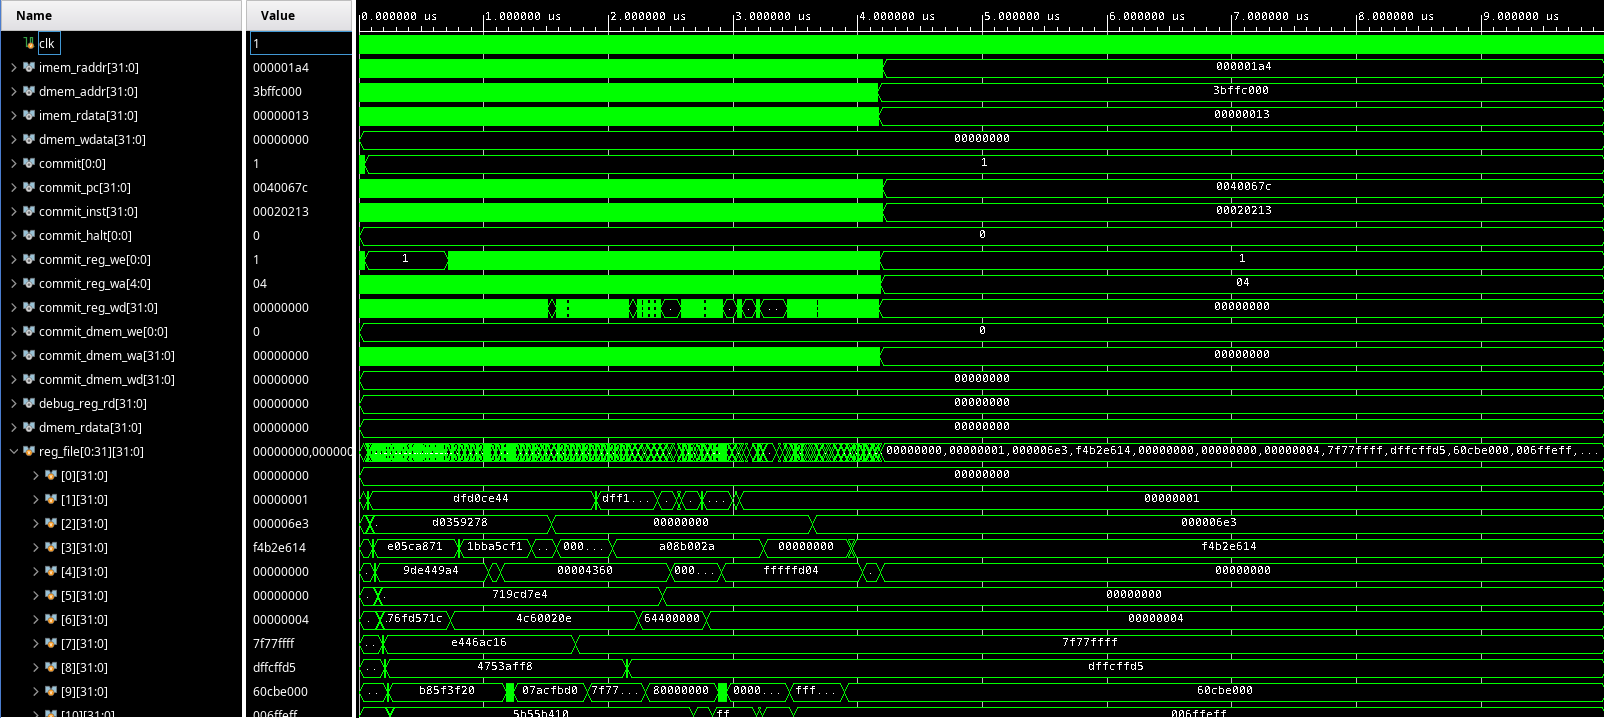
\includegraphics[scale=0.4]{pic/1-1.png}
    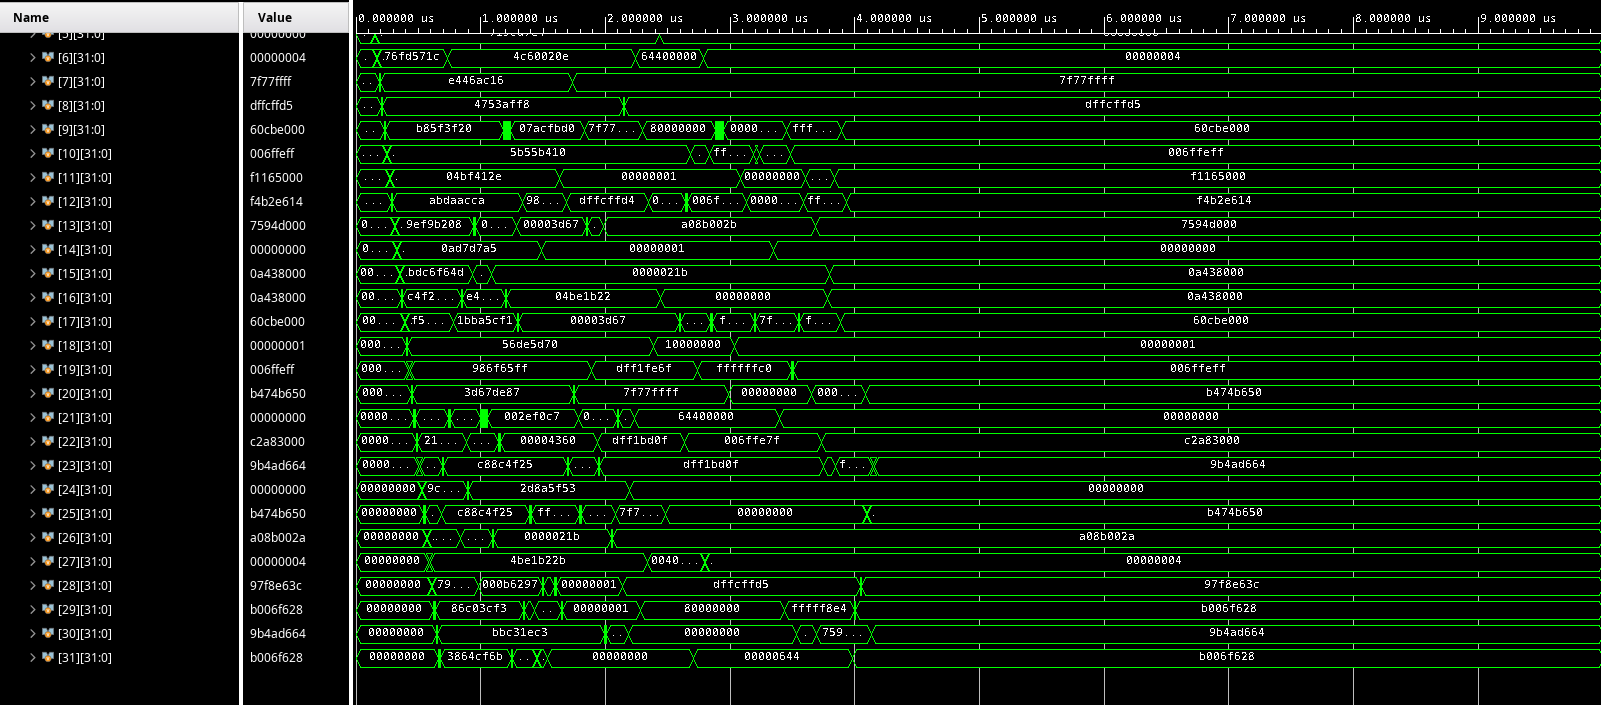
\includegraphics[scale=0.4]{pic/1-2.png}
    \caption{仿真结果}
\end{figure}
\begin{figure}[H]
    \centering
    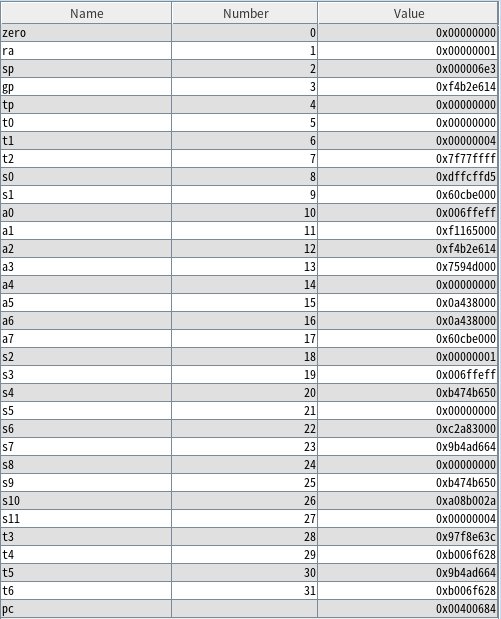
\includegraphics[scale=0.8]{pic/1.png}
    \caption{运行结果}
\end{figure}
可以看到,仿真结果和运行结果吻合的很好。
\subsection{Test2}
\begin{figure}[H]
    \centering
    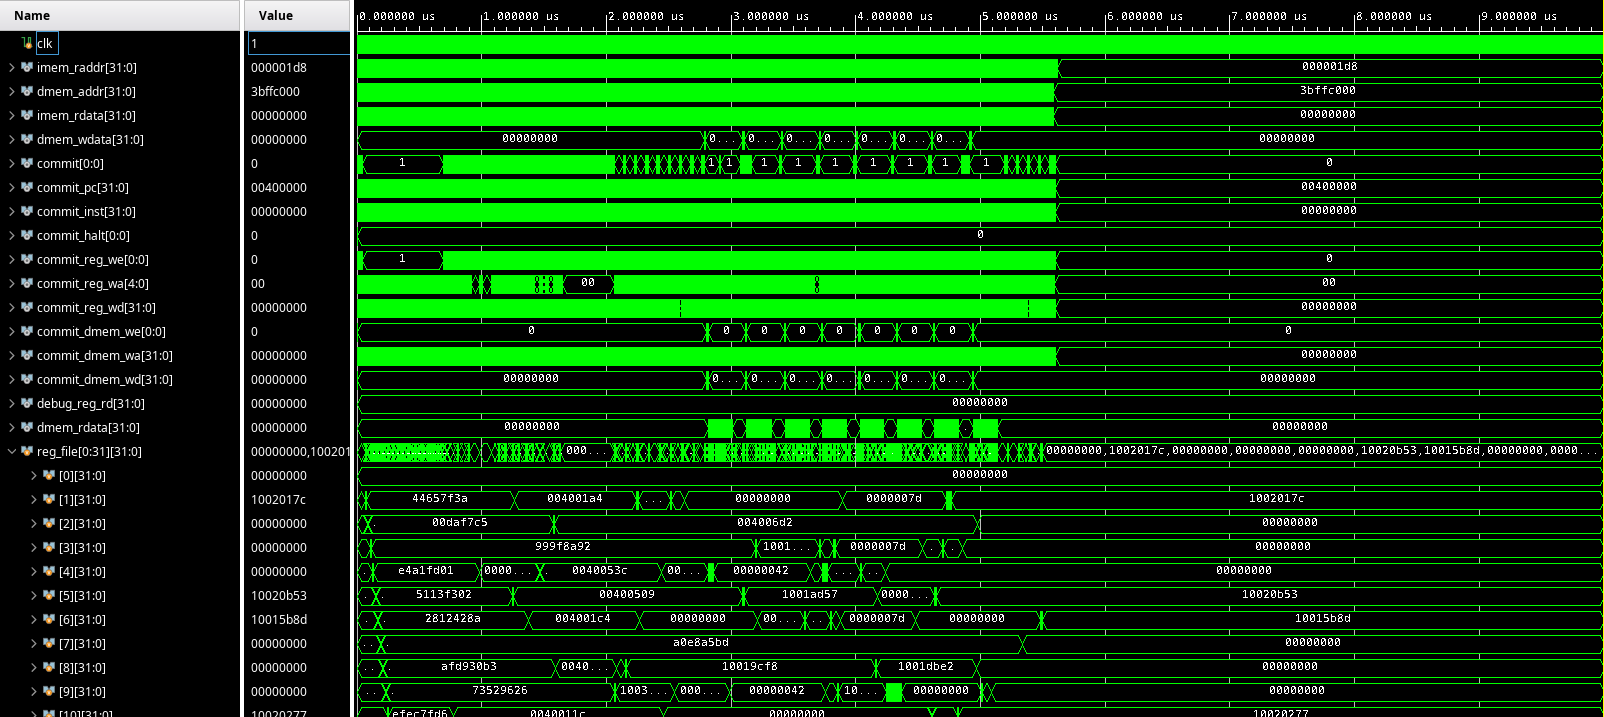
\includegraphics[scale=0.4]{pic/2-1.png}
    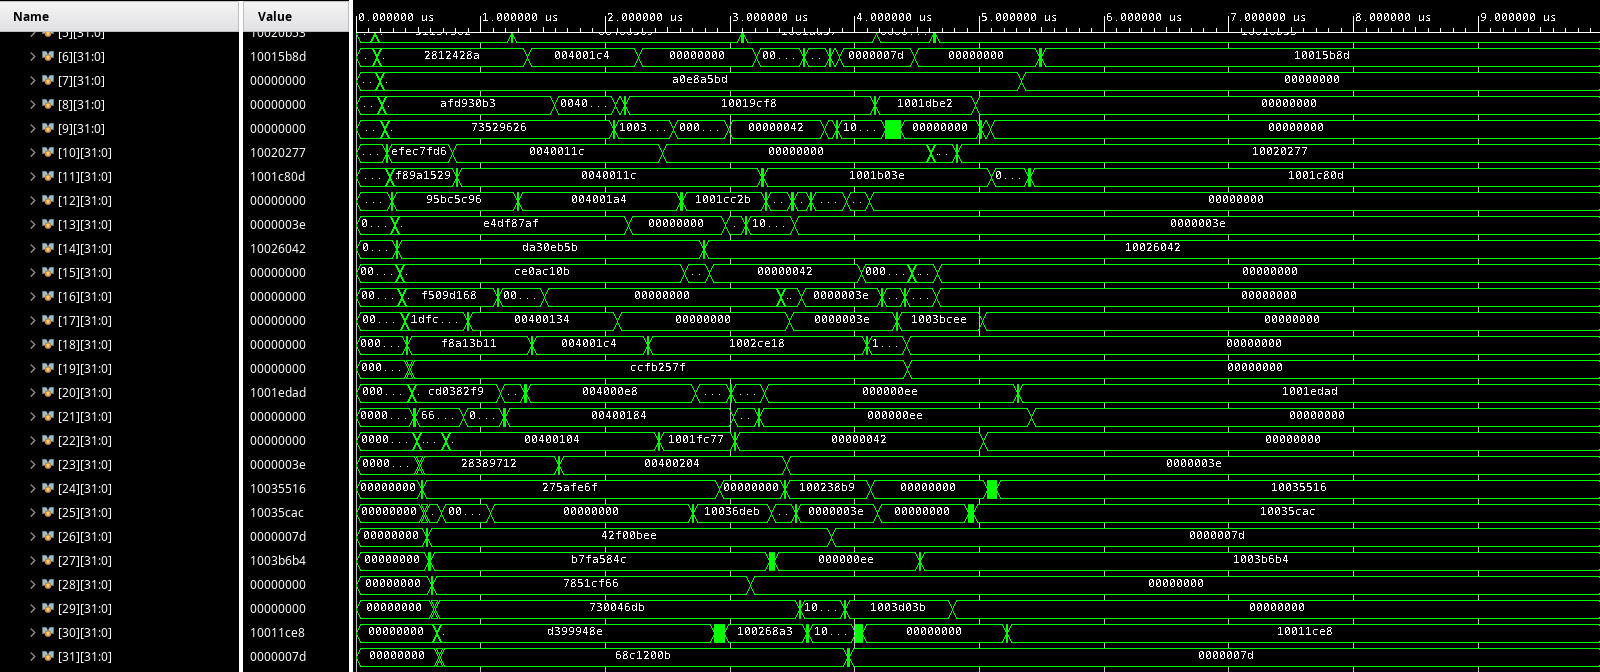
\includegraphics[scale=0.4]{pic/2-2.png}
    \caption{仿真结果}
\end{figure}
\begin{figure}[H]
    \centering
    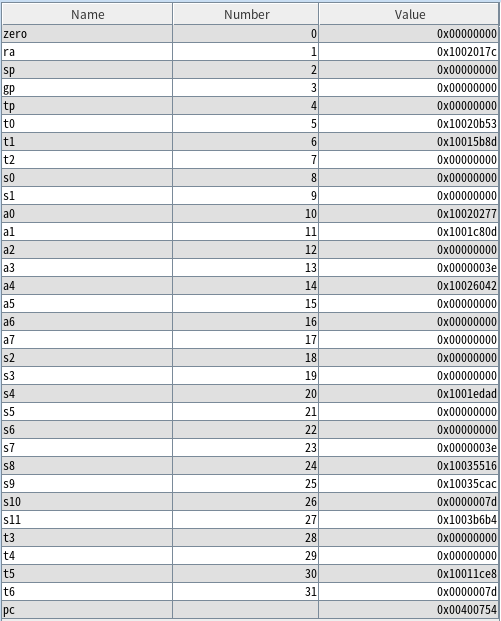
\includegraphics[scale=0.8]{pic/2.png}
    \caption{运行结果}
\end{figure}
可以看到,仿真结果和运行结果吻合的很好。
\section{电路设计与分析}
\subsection{前递模块}
\begin{figure}[H]
    \centering
    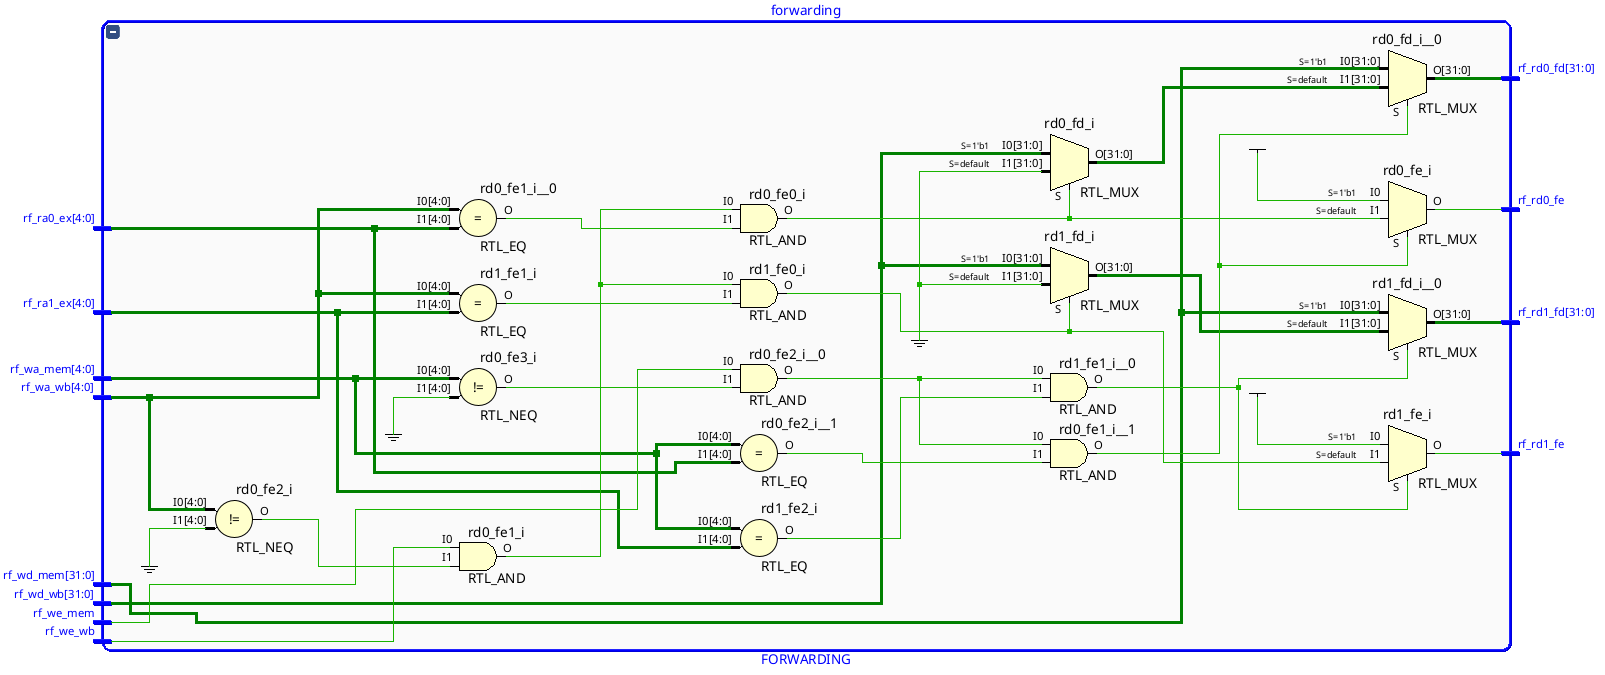
\includegraphics[scale=0.4]{pic/1pic.png}
    \caption{前递模块}
\end{figure}
\subsection{段间寄存器控制模块}
\begin{figure}[H]
    \centering
    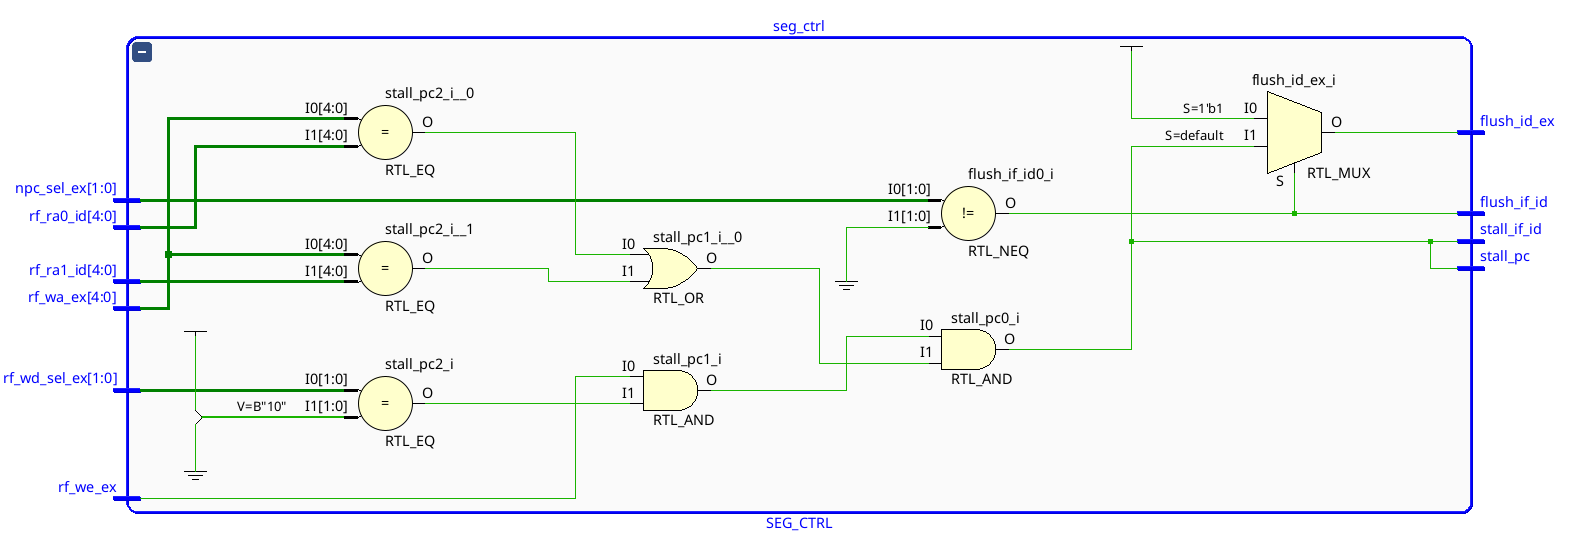
\includegraphics[scale=0.4]{pic/2pic.png}
    \caption{段间寄存器控制模块}
\end{figure}
\subsection{CPU模块}
\begin{figure}[H]
    \centering
    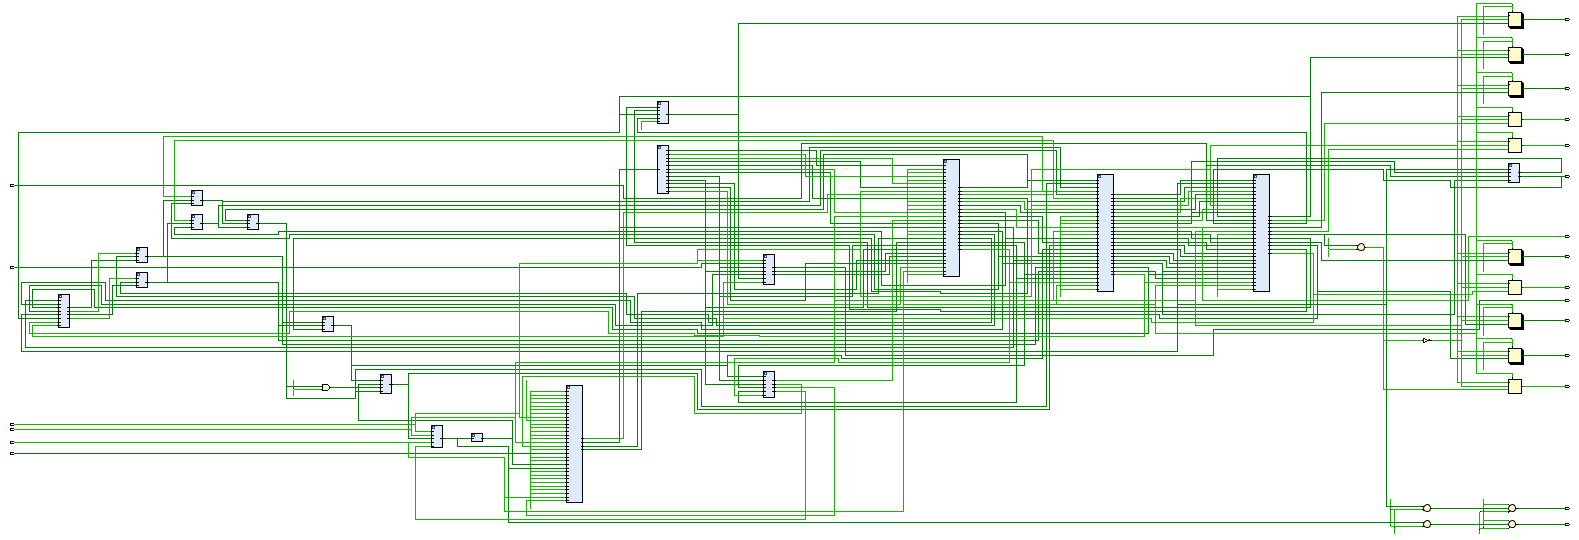
\includegraphics[scale=0.4]{pic/cpu.png}
    \caption{CPU模块}
\end{figure}
\section{测试结果与分析}
\subsection{Test1}
\begin{figure}[H]
    \centering
    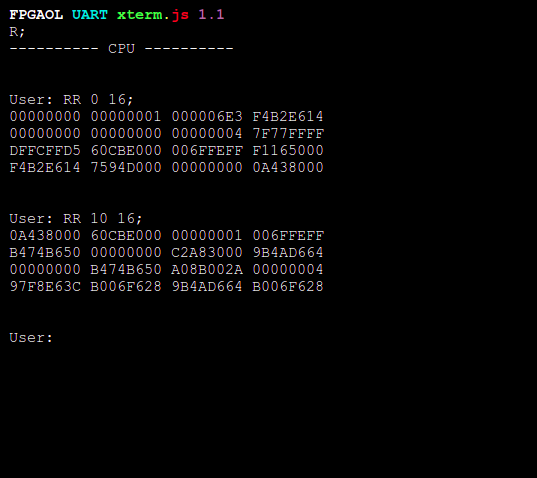
\includegraphics[scale=1]{pic/1_1.png}
    \caption{上板运行结果}
\end{figure}
可以看到,上板结果和运行结果吻合的很好。
\subsection{Test2}
\begin{figure}[H]
    \centering
    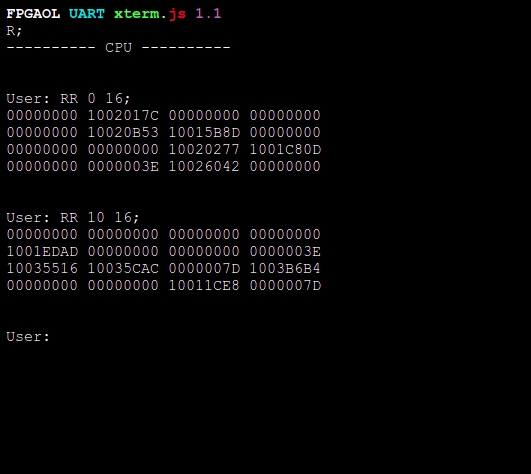
\includegraphics[scale=1]{pic/2_1.png}
    \caption{上板运行结果}
\end{figure}
可以看到,上板结果和运行结果吻合的很好。
\section{总结}
本次实验实现了前递模块与段间寄存器控制模块,并将其加入CPU模块,从而实现了一个完整的五级流水线CPU。
\end{document}